\chapter{Introduction} % 10316 characters

\section{Overview of the thesis} % 846 characters
\paragraph{\Cref{ch:ant}: \nameref{ch:ant}}
The development begins with a review of the algorithm.
For this, the original developers were to great help.
The system specifications were made and the details were discussed about the exact hardware and parts.
In this chapter, the previous works are presented, and the system is introduced.

\paragraph{\Cref{ch:plan}: \nameref{ch:plan}} 
This chapter describes the work that is done with all the errors and dead ends.
The desired hardware had some issue, and change through the project, as well as the software part.
Lots of possible solutions are raced to each other, considering both development cost and applicability.
There is also the ever-changing market of image processing.
The development tools were changed during the project several times.

\paragraph{\Cref{ch:results}: \nameref{ch:results}} 
In this chapter are listed all the codes and systems that are working.
There is also a detailed description of every step of the resulting processes, as well as the measurement of the resource requirement and timing.

\paragraph{\Cref{ch:sum}: \nameref{ch:sum}} 
In the last chapter, the questions and tasks given in the thesis proposal are answered.

\section{Background}
\paragraph{} % 515 characters
The usage of the UAVs (Unmanned Aerial Vehicle) grows in popularity.
The usability and the entertainment factor draws in more and more people, and the UAVs fill-up the aerospace.
Tough this is dangerous, there are little or no regulations regarding the drone flights (REGULATION (EU) 2018/1139; 4/1998. (I. 16.) Korm. rendelet).
The already existing regulations are old and not ready to handle such aerial traffic, thus prevent property or personal damage.
To prevent these, engineering solutions should be introduced.
A most common solution is to detect the closing danger with the already installed camera.

\subsection{Image Processing} % 2296 characters
The image processing tasks require huge computational power for image processing and detecting algorithms.

The most common way to store image data is a raster view.
An image consists of a grid with a width and a height.
This gives the main dimension of the image.
Every grid position represents a pixel with a value.
If the grid is one layer deep, the values show only the intensity of the pixel.
However, if 3 grids are present adjacent, then 3 different values can be represented. corresponding to the colours.
It can either by RGB (Red Green Blue) or HSV (Hue Saturation Value) as the most common two (\cref{fig:col_space}), but there are also many other pixel representations as well.

\begin{figure}
    \centering
    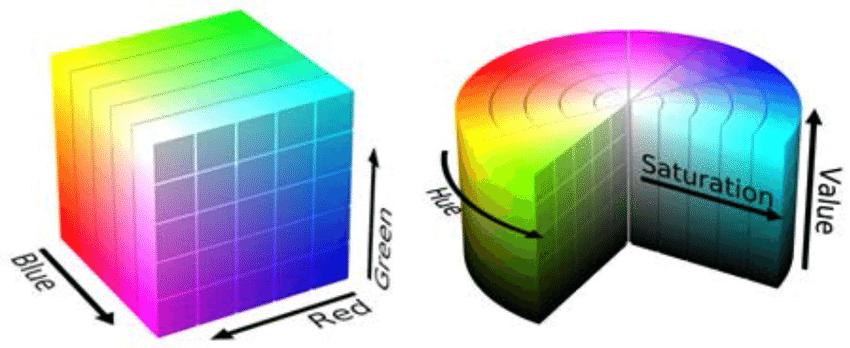
\includegraphics[width=\linewidth]{images/RGB-HSV-color-spaces.png}
    \caption{Comparison of the two most common color spaces (\cite{HVS-RGB})}
    \label{fig:col_space}
\end{figure}

By adding more layers more data can be displayed, such as an alpha channel, which makes the image transparent.
Representing the pixel values has also a couple of methods.
It can also be represented as an integer number or floating-point.
For integer representation usually, 8 bits are used, allowing the values to be between 0 and 255.
This is enough for the human eye to blend the represented image spectrum as a continuous space.
The computer algorithms are however too precise for such low representation therefore a floating-point value is used.
This can be range from 0 to 1 and can take up any value between based on the precision.

The raster representation can be easily displayed, but hard to gather information from it.
For this, the image either should be transferred to the other representation, or pixel-wise information should be extracted by specialised methods.
Converting the image representation can be computationally hard, for example, the Fourier transformation, or the Hough \cite{Duda:1972:UHT:361237.361242} transformation.

The other option is the convolution implementation.
This mathematical formula goes like:

\begin{equation}
    g(x,y) = h(x,y)\star f(x,y) = \sum_{k=-\infty}^{\infty} \sum_{l=-\infty}^{\infty} h(x-k,y-l) f(k,l)
\end{equation}

where g is the output image f is the input image and h is a convolutional kernel.
The transformation is LSI (Linear Space Invariant), commutative, associative, distributive, and associative for scalar multiplications.
In the real-life, both h and f are finite size.
This entails the modifications of the equation,

\begin{equation}
g(x,y)=\sum_{k=1}^{height} \sum_{l=1}^{width} h(k,l) f(x+k-1,y+l-1)
\end{equation}

however, the convolutional filter is usually larger than 1 pixel, thus at the edges, an indexing problem arises.
For this, the image should be extended by $\lfloor size_h/2 \rfloor$.
To do this there is a couple of solution, as filling the missing part with zeros or constants, copying the last pixel of the image or wrapping the image around creating a torus from it (\cref{fig:borders}).

\begin{figure}
    \centering
    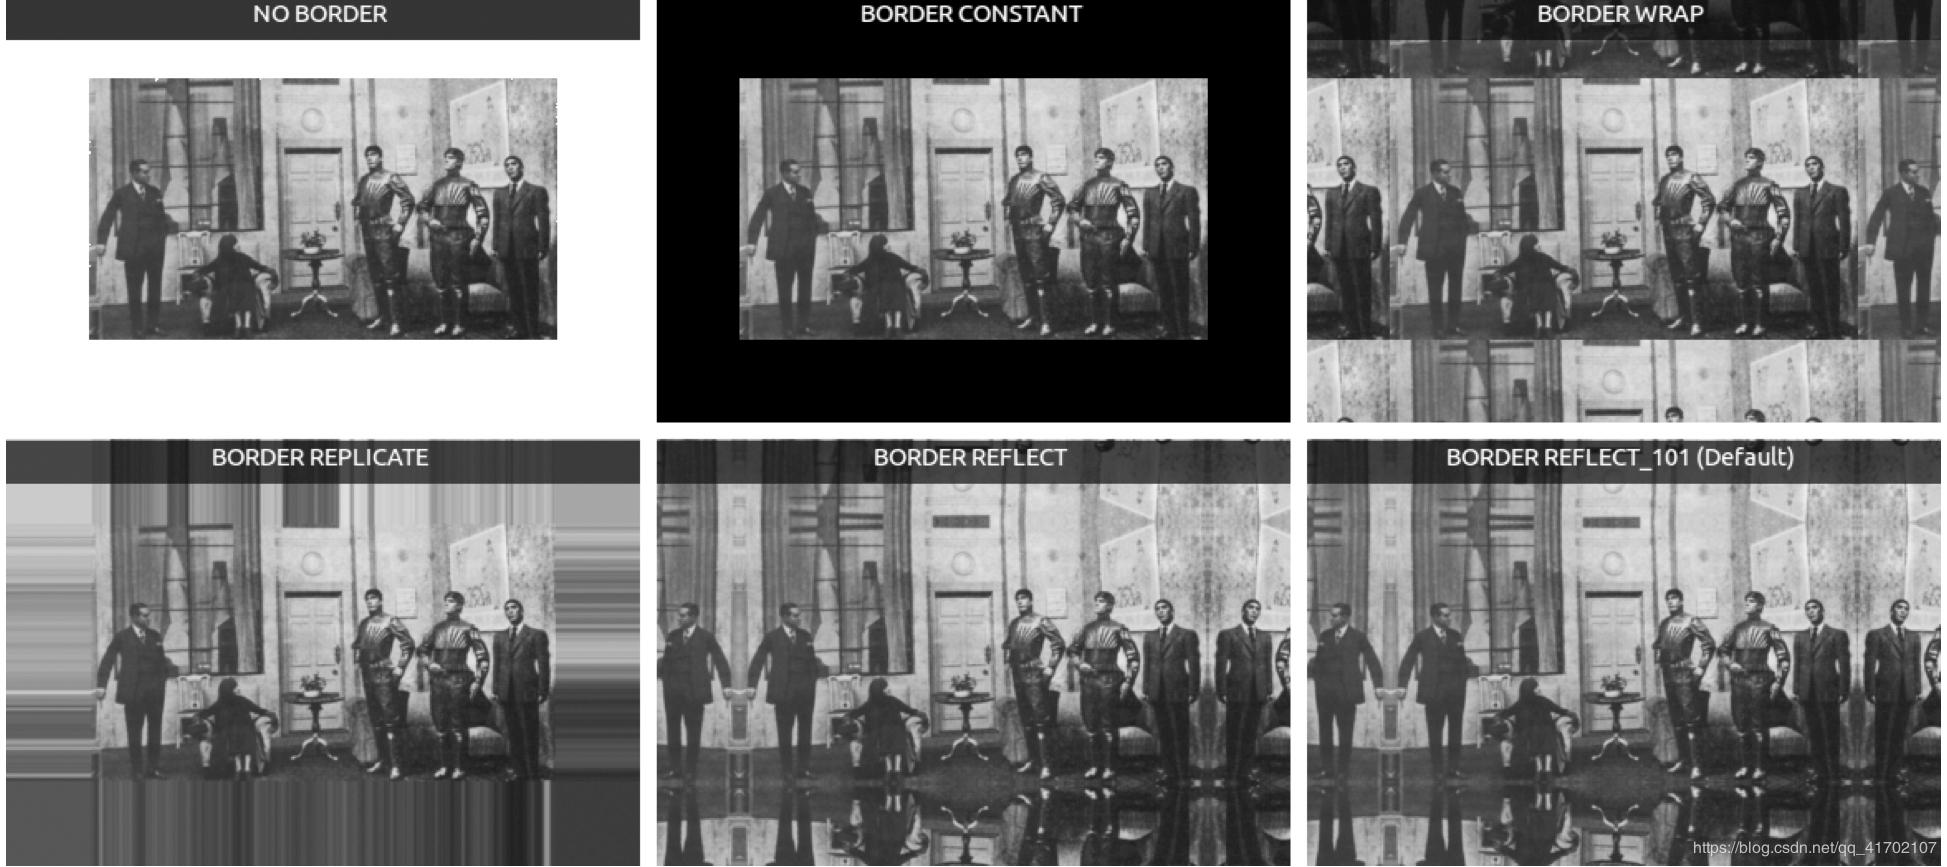
\includegraphics[width=.9\linewidth]{images/borders.jpg}
    \caption{different border types in the OpenCV library \cite{img_border}}
    \label{fig:borders}
\end{figure}

The convolution can be used for different applications, based on the kernel it uses.
As not only the central pixel is considered but the neighbouring values as well, the resulting image transforms in relation to the environment of each pixel.
It can smooth the image, can enhance the edges or blur.

% The greatest advance in the convolution was when as a neural network, the kernel weights was set by a deep learning algorithm.

\subsection{Neural network} % 3742 characters
Deep learning is a buzzword, in the IT industry, for almost a decade.
This is a Machine learning method, for applications where the usual algorithmic approach is not possible.
The basic idea is to copy the learning mechanism of the human brain.
There is a learning set, with some input structure and the corresponding expected result.
The system starts from a random inner state and calculates the outputs.
After a comparison of the expected and actual results, the inner state is updated.
Thus the inner state adjusts step by step to the target function.
For this 3 component is required.
An underlying pattern, which can be approximated by the network, a learning set, to train the network, and a complex mathematical representation that is hard to implement.

Deep learning is a common solution for image classification, since the correlation of the pixels, and the meaning behind the picture is hard to describe through mathematical functions.
For that matter, we also know that the pattern exists, as even a kid can recognise basic shapes and even more complex forms on the image.
The only thing missing is the training dataset and a proper working neural network to learn.
The first approach for image procession was the fully connected network.
In a traditional fully connected network all the inputs are connected to each other.
A pixel of an image has few in common with the other pixels except the closeby neighbours.
This results in lots of computations that have little impact on the final result.
The other problem if the images have some offset.
A fully connected layer considered the exact position of the pixel as an important parameter.
To process the image efficiently a convolutional neural network should be used.

The previously introduced mathematical formula can be easily modified to work as a neural network.
The convolution considers only the kernel size area of a pixel, eliminating noise that was introduced by the presence of the further pixel.
Since all the calculation that should be done is limited to the kernel size, it also uses fewer resources.
The convolution is also capable of changing the dimensions of the image.
Meaning that the 3rd dimension that stores the colour data can be expanded to store other features.
In a convolution operation, there can be more layers of an image, each containing different features.
These features are not always has some physical meaning rather some abstract representation of the image, on which, later decisions depend (\cref{fig:convolvution}).

\begin{figure}
\centering
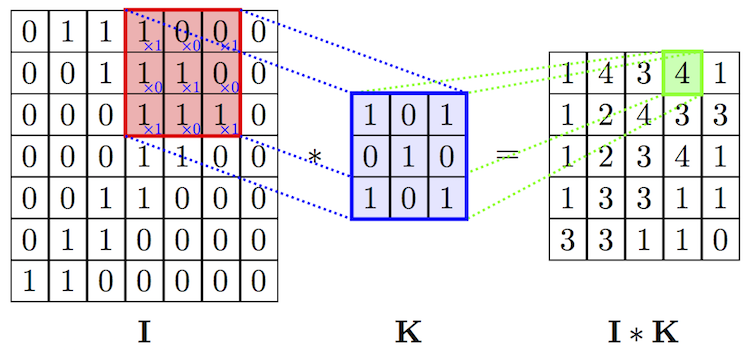
\includegraphics[width=\linewidth]{images/convolve.png}
\caption{Visualisation if the convolution \cite{spark_deep_nodate}}
\label{fig:convolvution}
\end{figure}

The kernel stride determines how small the output image will be.
On every stride step, one pixel is calculated, hence if the stride is 2 then every $2^{nd}$ pixel is calculated.
This makes the output image half of the size of the input image.
This is not a problem for such a system since the required information is not graphical, thus if the smaller image can store the information the fewer resources should be used.

A convolutional layer being an LSI system, can not be chained due to the linear property.
To chain more convolution together the system needs to become nonlinear.
To provide the nonlinearity to the system activation functions are used.
These are nonlinear functions that wired to the summation expression of the layer.
The function can be complex like a sigmoid function or can be a plain rectified linear unit (ReLU).
This ReLU function is a linear function on the positive halfplane, and zero on the negative (\cref{fig:relufunc}).
This property makes it easy to calculate, but still providing the required nonlinear property.

% ReLu
\begin{figure}
\centering
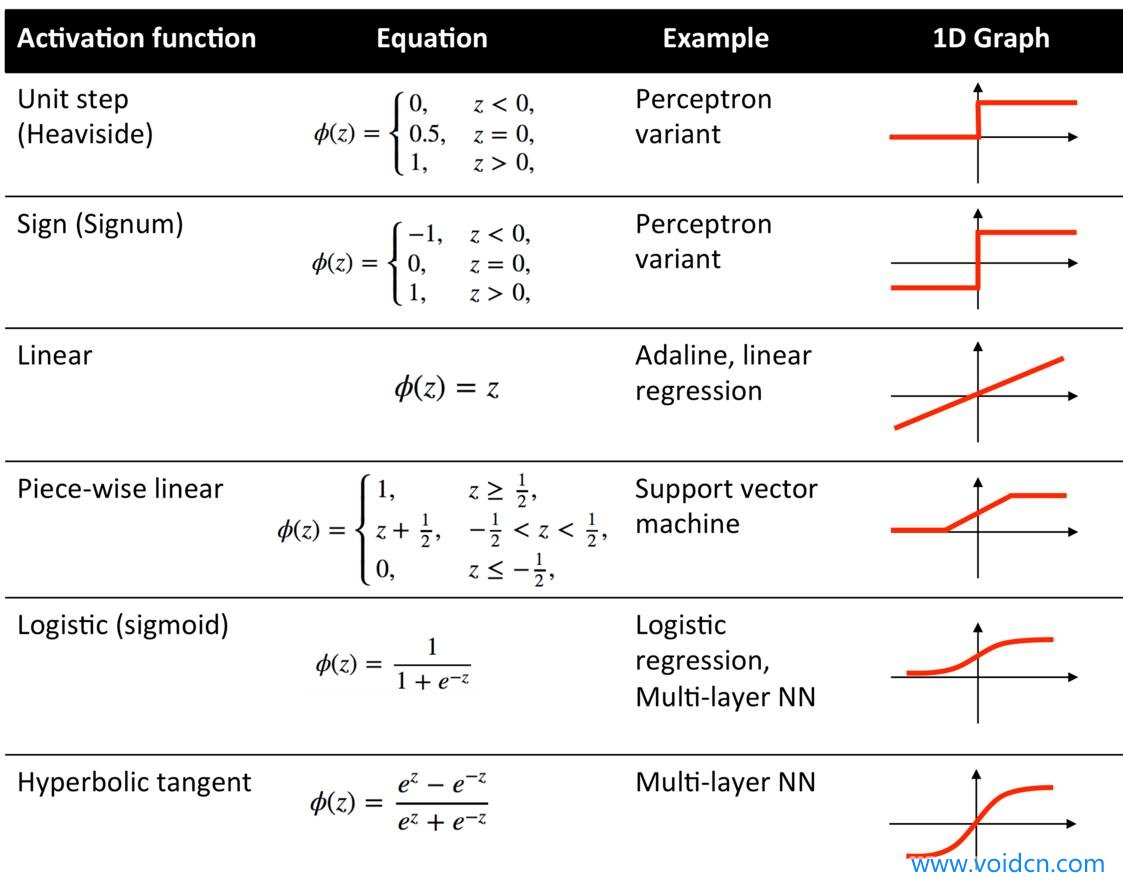
\includegraphics[width=.85\linewidth]{images/activation-functions.jpg}
\caption{examples of possible activation functons in a neural network \cite{sebastian_activation} }
\label{fig:relufunc}
\end{figure}

In a CNN architecture, there is usually another function is implemented.
This function also adds nonlinearity to the system and also raises the most prominent features.
The so-called pooling layer also uses a kernel which strides through the images and replaces the pixel values according to the kernel.
Usually, max-pooling is the most common.
This returns the maximal value inside the kernel.
There are also other types of pool functions like average, or $l^2$ norm pooling.

To do the final decision a fully connected layer is required.
This layer transforms the grid-like values to an array or a single number.
But instead of weighting the pixel values, now it weights features extracted by the previous layers.
Usually, an array is preferred, where the array elements are all the possibilities of a certain output.
The array can be considered the confidence of the network.
This is called One hot encoding

\subsection{FPGA} % 2917 characters
The drones, due to weight limits, unable to carry large power sources, and the computing devices should also be small, light and energy-efficient, hence the GPUs (Graphical Processing Unit) are out of the picture.
Another possible computing platform is the FPGA (Field Programmable Gate Array), more specifically the SoC (System on a Chip).

The FPGA is a circuit consist of a series of logic gates and the programmable interconnects between the gates (\cref{fig:fpga_block}).
The strength of such a circuit lies in its programmability.
With basic logic gates, every function can be implemented.
After designing the function and assembling the logic gates, the final circuit can execute the required calculations and produce the results.
In the traditional development phase, the circuit was implemented in a semiconductor.
In case of an FPGA however, the silicon parts are already in place, only by programming the connections every circuit can be implemented.

The system implemented on an FPGA will of course never be as fast as an ASIC (Application-Specific Integrated Circuit) optimised for the exact task.
On the other hand, the FPGA has not to be reworked from scratch every time a new task is at hand.
Designing new software to program the interconnects, does require less time and less expensive.
An FPGA can also be used for different purposes based on the program.
In comparison to the classical processing algorithms, the FPGA does not use a finite ISA (Instruction Set Architecture), but a low-level gate array.
This gate array can work faster, and can even implement functionalities that are hard or not possible with a traditional SISD (single instruction stream, single data stream) architecture.

\begin{figure}
    \centering
    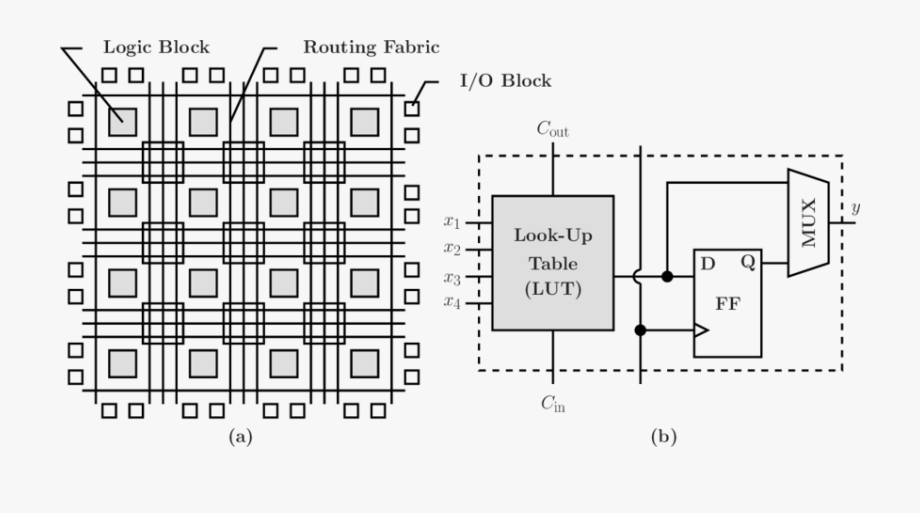
\includegraphics[width=\linewidth]{images/fpga-block-diagram.png}
    \caption{Block diagramm of an FPGA (\cite{fpga_block})}
    \label{fig:fpga_block}
\end{figure}

FPGAs can be easily adapt to specialised tasks, but some tasks are not optimal, or hard to implement on programmable logic.
Therefore the modern architectures are usually designed with Processor systems included.
This means that the silicon slice has a dedicated part where fixed hardware is implemented.
This reduces the area of the PL part but allows the whole silicon to work both as an FPGA or a PS as requested, in most cases as both at the same time.
The Xilinx\texttrademark product line named there SoC products ZYNQ.
There are several configurations and builds for this chip family.
For the cheaper devices, the SoC contains an Artix\texttrademark or Kintex\texttrademark FPGA, which are both available separately, and an ARM cortex A-series chip.
This setup is easy to design since the two subsystems are placed side by side each other.
The higher-grade devices however required to design the whole FPGA part specifically for the device.
These FPGA parts are resembled greatly to the other Ultrascale\texttrademark and Ultrascale+\texttrademark standalone FPGAs but modified some ways.
The higher-end devices also can contain some special parts like R-series ARM\texttrademark processors for Real-Time applications, video codec hardware, of radiofrequency and telecommunication systems.
There are also chips where a GPU is included on the silicon alongside the FPGA and the PS.
These architectures also integrate HBM (High Bandwidth Memory) on the same chip.
This ACAP (Adaptive Compute Acceleration Platform) system contains everything for accelerating a modern computational system.
The special task implemented on the FPGA, the calculation tasks are done by the GPU, the cache and buffering loaded to the HBM and the system is controlled by the processor subsystem.
It combines the advantages of all parts without sacrificing efficient programming. 
This combined system called SoC.
The modern system also changed the basic gate implementations to CLB (Configurable Logic Block).
CLBs can solve more complex logic functions in there own by using LUT (Look Up Table) and contains register as well.
Thus the FPGA reduces the latency closed by the interconnects, and also can function as a memory or temporary storage.
There are also complex arithmetic units included in the CLBs like adders and multiplier units.
By using these bypasses the latency LUT accelerating the system even more.
In the interconnecting part are also implemented a carry propagation connection, which connects the CLBs carry logic parts.
Thus greater adder circuits can be implemented without the carry occupying the connection bandwidth.
DSP (Digital Signal Processor) slices also can be found among the logical blocks.
This block contains simple ALUs (Arithmetic-Logic Unit), accelerating the major algorithms and reducing the CLB requirements of the signal processor applications.
The configurable SoCs are also small in size and runs on low power.

The thesis discusses a system design that can read the camera images and detect the closing obstacle while running on SoC.

\clearpage % Ez azért kell, hogy nehogy képek átcsússzanak a következő fejezethez